\chapter{Methods}\label{ch:methods}
\section{The computing environment at LCLS}
- Include basics around the PSANA interface\\
- For example how the date is converted, then stored and\\
- the analysis opportunities along the way
- I think this will be a longer subsection since a lot of my work went into this and I'm regularly contacted about it.
- Short introduction what we have to go through\\
- Reminder of detectors and analysis environment
\subsection{PSANA - Python interaction with LCLS computing}
%%%
\section{pnCCD photon detectors}\label{sec:pnccd-corr}
- Describe signal on the pnCCDs\\
- Calibrations and corrections - use LAMP paper\\
- single hits\\
- multiple hits
\subsection{Signal analysis}
- Present data from 1500eV photon energy on Xe backfilled chamber with the pnCCDs in spectroscopy mode to argue that the pedestal and offset corrections are enough to correct for fluoresence.\\
- Masked areas in image
%%%
\section{Combining multiple pnCCD detectors}
- Explain how I combined pnCCD detectors to perform reconstructions on it.\\
- Can reuse material from the LAMP pnCCD paper
%%%
\section{Hitfinding}
- Discuss the hitfinding.\\
- iTOF vs. pnCCD\\
- vs. Actual dynamics visible in diffraction images
%%%
\section{Phase retrieval from a single diffraction pattern}\label{sec:phase-retrieval}
- Short intro into phase retrieval
\subsection{The inverse problem: Phase retrieval}
%%%%%%%%%%%%%%
%- Introduce some aspects from phase retrieval algorithms.
%%%%%%%%%%%%%%
\begin{figure}
	\centering
		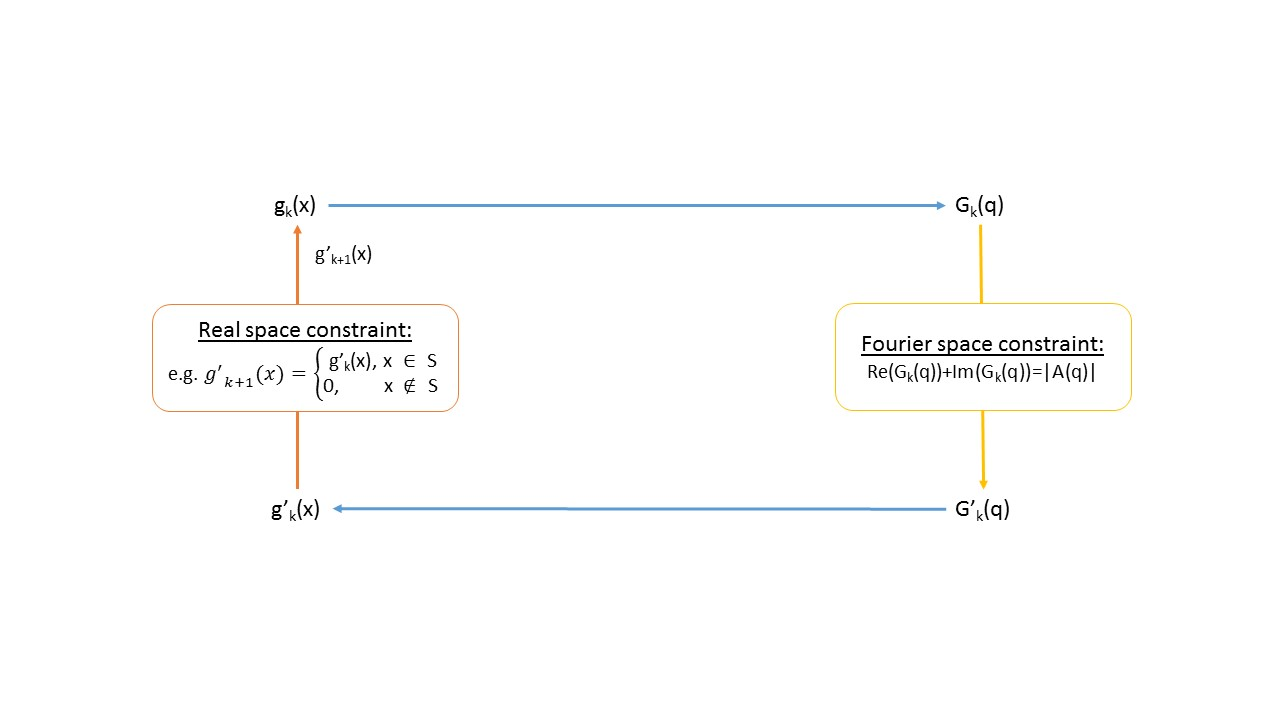
\includegraphics[width=1.00\textwidth]{images/phase-retrieval-algorithm.jpg}
	\caption[Example of a phase retrieval algorithm.]{Principle of a phase retrieval algorithm. The real space object $g_{k}\left(x\right)$ is Fourier transformed to $G_{k}\left(q\right)$. The function $G_{k}\left(q\right)$ is altered to fit the constraints set in Fourier space, hence $G'_{k}\left(q\right)$. $G'_{k}\left(q\right)$ is inverse Fourier transformed to $g'_{k}\left(x\right)$. After fulfilling the real space constraints the iterative starts again using $g_{k+1}\left(x\right)$. From \citep{Fienup-1982-AO}.}
	\label{fig:phase-retrieval-algorithm}
\end{figure}
The loss of the phase in the scattering process results ultimately in the recovery of the complex fields. The scattered intensity $I\left(\vec{Q}\right)$ is proportional to the form factors $\left|f^{0}\right|^{2}$. To recover the phase and thus reconstruct the particle iterative algorithms have been developed \cite{Fienup-1982-AO}. Figure \ref{fig:phase-retrieval-algorithm} illustrates such an iterative algorithm, where the image of an object $g_{k}\left(x\right)$ is Fourier transformed to reciprocal space $G_{k}\left(x\right)$ and then back again resulting in $g_{k+1}(x)$, while sufficing certain constraints.\\
The constraints are rather strict defined in the reciprocal space as they have to reproduce the actual measurement $I=A\cdot A^{*}$. The criteria that need to be met in real space can be chosen more freely. Generally, the recovered object should be physical, i.e. consist of positive values or should be of a certain (known) size. In simplified terms, one can introduce a support structure $S$ that meets the physical constraints and can therefore be used to, for example, zero outling values. Throughout the iterations the functions $g_{k}(x)$ evolve and eventually converge into a solution. If one uses the above criterion, one can show that the error between the reconstructions and the actual measurement continuously reduces, which is why it is commonly referred to as error-reduction algorithm \cite{Fienup-1978-OL}.\\
It should be noted that there is a great variety of manipulations that can be done upon not fulfilling a realspace constraint and although their function is fairly similar there is a great variety of algorithms. Worth mentioning is the hybrid input-output (hio) \cite{Fienup-1978-OL} and the relaxed averaged alternating reflection (RAAR) \cite{Luke-2005-IP}.
%
%
%
%
%\subsection{Solving the inverse problem}
\subsection{2D reconstructions and limitations}
\subsubsection{Hawk program}
- Describe Filipe's program
\subsubsection{Resolution enhancement through combination of rear and front pnCCD}
- Showcase difference of rear pnCCD only vs. front + rear pnCCD vs. front + rear pnCCD 'cropped' for best results. Recycle work from LAMP pnCCD paper
\subsection{1D reconstructions}
- Describe my algorithm in 1D in detail
%%%
%\section{Signal on time of flight detector}
%- Explain what we see in Xe, He and XeHe sample environments.\\
%- and further analysis aspects, e.g. Aqiris / psana interface.
%%%
\section{Summary of methods}
- Comprehensive summary 